\documentclass[biblatex,aspectratio=169,11pt]{mybeamer}

\usetikzlibrary{backgrounds,calc,decorations.pathreplacing,fit,matrix,patterns,positioning,shapes,shapes.multipart,tikzmark}
\makeatletter
\let\@@magyar@captionfix\relax
\makeatother

%Add page footer
\setbeamertemplate{footline}[text line]{%
  \parbox{\linewidth}{\vspace*{-8pt}\hfill CS6290 Privacy-enhancing Technologies\hfill\insertpagenumber}}
\setbeamertemplate{navigation symbols}{}

\title{A Preliminary Study on Stateless Blockchain}
\author{Yang Ji}
\date{April 15, 2019}

\addbibresource{ref.bib}

\begin{document}

\maketitle%
\PrintTOC%

\section{Introduction}

\begin{frame}{Background}
  \begin{itemize}
    \item In cryptocurrency, peer-to-peer payment transactions are asynchronously broadcasted and recorded in an ordered ledger.
    \item Consensus protocol requires nodes to validate new transactions. 
    \item e.g. To send 6 ETC from Alice to Bob requires that Alice has at least 6 ETC.
    \item Simply querying the history from adjacent nodes is infeasible and insecure due to the large size of blocks.
    \item For that reason, most cryptocurrency nodes need to locally maintain the \alert{ledger state}, which means downloading all past transactions/accounts.
  \end{itemize}
\end{frame}

\begin{frame}{Background}
  \begin{itemize}
    \item In Bitcoin, Zcash and Komodo, \alert{validation state} is a set of immutable coins called \alert{UTXO} (unspent transaction output)
  \end{itemize}
  \vspace{-1em}
  \begin{figure}
    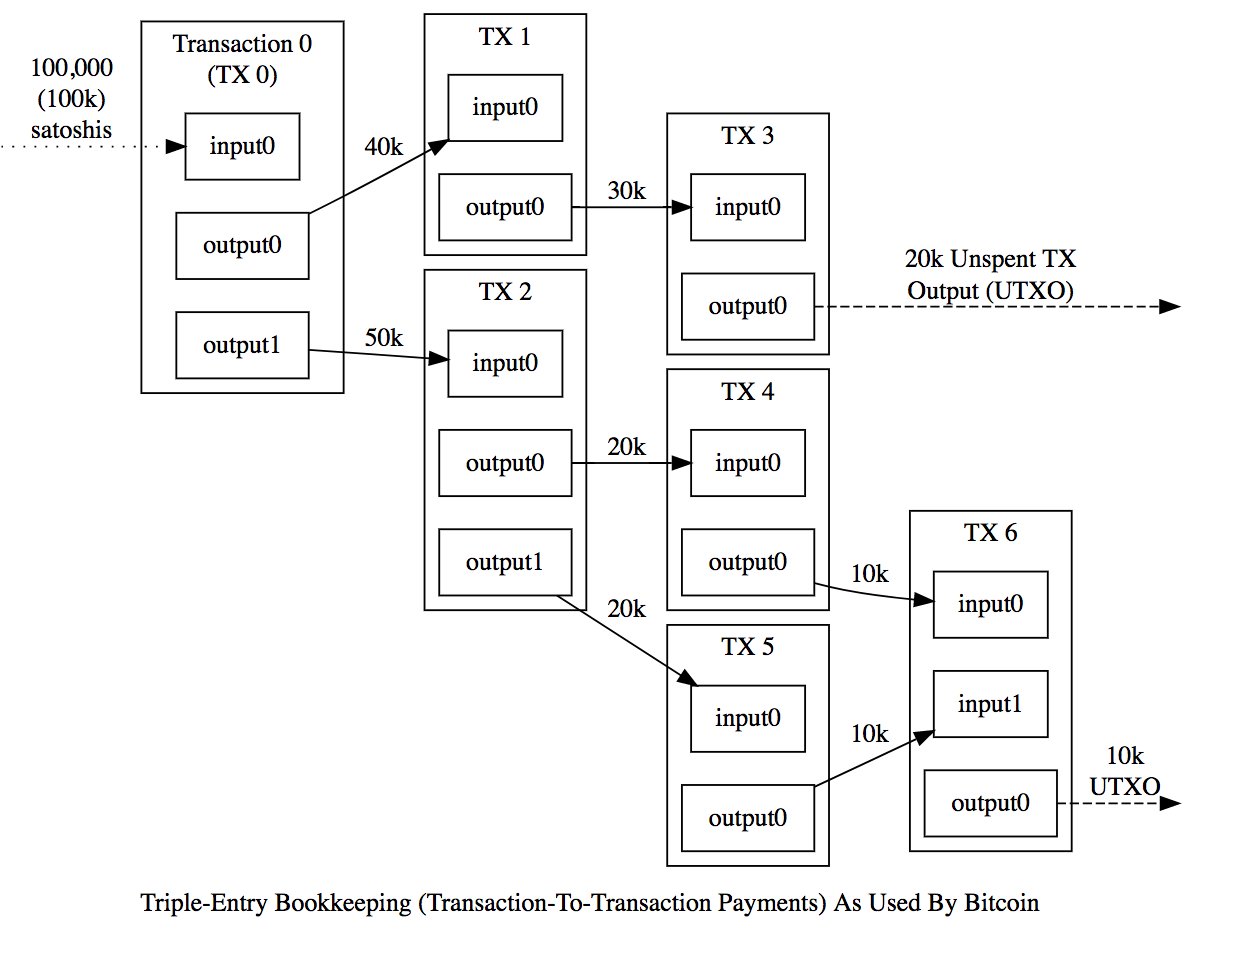
\includegraphics[width=0.45\linewidth]{figs/utxo.png}
    \caption{UTXO Model}
  \end{figure}
\end{frame}


\begin{frame}{Background}
  \begin{itemize}
    \item In Ethereum, Nxt and Bitshares organize \alert{validation state} as a set of mutable (and potential long-living) \alert{accounts}.
  \end{itemize}
  \vspace{-1em}
  \begin{figure}
    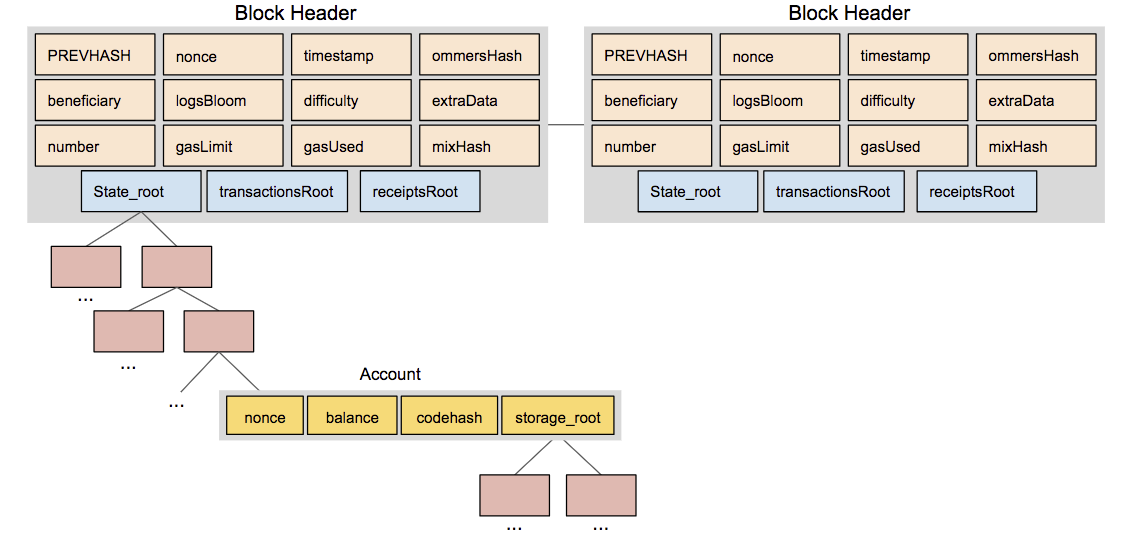
\includegraphics[width=0.7\linewidth]{figs/account.png}
    \caption{Account-based Model}
  \end{figure}
\end{frame}

\begin{frame}{background}
  \begin{itemize}
    \item Other cryptocurrencies
  \end{itemize}
  \vspace{-1em}
  \begin{figure}
    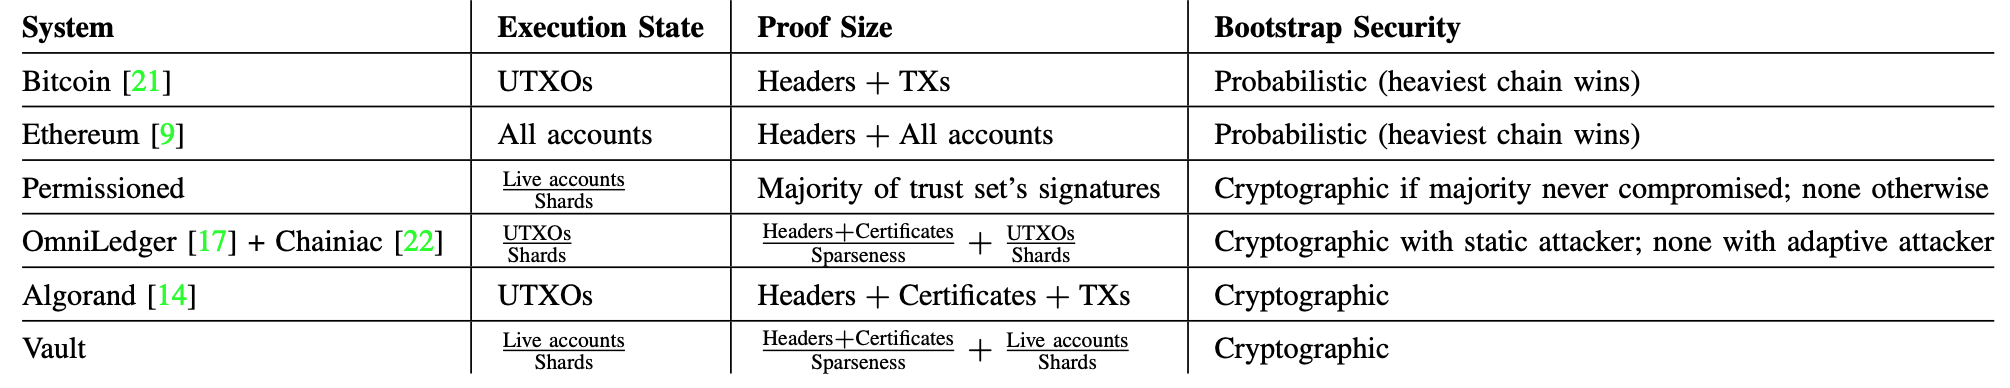
\includegraphics[width=0.9\linewidth]{figs/summary.png}
    \caption{Comparison of different cryptocurrency models }
  \end{figure}
\end{frame}

\begin{frame}{Motivation}
  \begin{itemize}
    \item Maintaining ledger state is cumbersome from the perspectives of \alert{storage} and \alert{bootstrapping}
    \begin{itemize}
       \item Large size (Bitcoin is around 150 GB and Ethereum has exceeded 400 GB)
       \item Data storage size is linear with block number and could grow substantially in the coming years
       \item Slow disk I/O operations (LevelDB or RocksDB)
       \item DoS attack (adversarially-crafted transactions that need massive of disk accesses)
       \item Increase the possibility of centralization in blockchains.
    \end{itemize}
    \item It thus appears that we need to remove the \alert{ledger state} and allow miners to validate pending transactions without storing all past blocks. 
  \end{itemize}
\end{frame}

\begin{frame}{Stateless Blockchain}
   \begin{itemize}
    \item This design concept of \alert{Stateless Blockchain} is referred to Peter Todd's blog post~\cite{Tod}. 
    \item Nodes might participate in transaction validation without storing the entire state of the ledger.
    \item Several people including Peter Todd and Mike Hearn also talked about stateless clients for Bitcoin in 2013. Back to then, they call it \alert{Storageless}.
    \item Many optimized schemes are put forward in the forum, such as Merkle Mountain tree~\cite{MMR} and asynchronous accumulator~\cite{reyzin2016efficient} for dual accumulator.
  \end{itemize}
\end{frame}

\section{Existing works}

\begin{frame}{Categories}
  \begin{itemize}
    \item Method 1: \alert{Storage rent}
    \item Method 2: \alert{Sharding}
  \end{itemize}
\end{frame}

\nocite{*}
\PrintRef%
\PrintQA%

\end{document}
